% Four-page anonymous review draft. Check the current CVIS Overleaf template before submission.
\documentclass[letterpaper,10pt]{article}
\usepackage[T1]{fontenc}
\usepackage{times}
\usepackage[left=0.8in,right=0.8in,top=0.7in,bottom=0.7in,columnsep=0.3in]{geometry}
\usepackage{amsmath,amssymb,booktabs,graphicx}
\usepackage{tikz}
\usetikzlibrary{arrows.meta,positioning}
\usepackage{caption}
\captionsetup{font=small,labelfont=bf}
\usepackage[hidelinks,pdfauthor={},pdftitle={Profiled Joint Subset Search (PJSS) for Sparse Equation Discovery from Noisy Trajectories}]{hyperref}
\setlength{\parindent}{1em}
\setlength{\parskip}{0pt}
\setlength{\textfloatsep}{10pt}
\setlength{\abovecaptionskip}{4pt}
\setlength{\belowcaptionskip}{1pt}
\newcommand{\lead}[1]{\par\smallskip\noindent\textbf{#1}\ }
\newcommand{\R}{\mathbb R}
\makeatletter
\renewcommand\section{\@startsection{section}{1}{\z@}{-2.1ex plus -0.4ex minus -0.2ex}{0.9ex plus 0.2ex}{\normalfont\large\bfseries}}
\renewcommand\@seccntformat[1]{\csname the#1\endcsname.\quad}
\makeatother
\newcommand{\LorenzCoef}{0.66}
\newcommand{\LorenzShort}{0.038}
\newcommand{\LorenzLong}{0.600}
\newcommand{\LorenzExact}{1}
\newcommand{\RosslerCoef}{0.25}
\newcommand{\RosslerShort}{0.060}
\newcommand{\RosslerLong}{0.095}
\newcommand{\RosslerExact}{1}
\newcommand{\ChenCoef}{1.93}
\newcommand{\ChenShort}{0.008}
\newcommand{\ChenLong}{0.015}
\newcommand{\ChenExact}{1}
\newcommand{\LorenzEqX}{-10.084x +10.110y}
\newcommand{\LorenzEqY}{27.844x -0.989y -0.994xz}
\newcommand{\LorenzEqZ}{-2.668z +1.003xy}

\raggedbottom
\begin{document}
\begin{center}\vspace*{0.13in}
{\large\bfseries Profiled Joint Subset Search (PJSS) for Sparse Equation Discovery\\from Noisy Trajectories\par}
\vspace{0.08in}\end{center}
\begin{center}\textbf{\large Abstract}\end{center}
\noindent\textit{We study recovery of sparse differential equations from one noisy trajectory. Profiled Joint Subset Search (PJSS) alternates joint estimation of states and coefficients with a search for better combinations of equation terms. A local quadratic model accounts for trajectory adjustment, screening many supports before nonlinear refitting. Sparsity is selected using a BIC-inspired score with fixed development-selected defaults. Across 77 in-library chaotic systems, PJSS recovers exact support in 89.0\% of runs, including 85.3\% on 49 systems outside development benchmarks. On 64 paired runs from 35 new systems, it recovers 53, compared with 36 or 41 for DEDi under two selection rules. New fixed-case illustrations show recovered equations, held-out predictions and autonomous attractor geometry. Ablations attribute the larger gain to subset proposals and a smaller gain to profiling. The main evidence concerns simulated, fully observed systems; measured-data tests expose failures.}

\vspace{5pt}
\noindent\begin{minipage}[t]{0.478\textwidth}\vspace{0pt}
\section{Discovering equations from measurements}
A noisy trajectory can support several sparse models. Correlated candidate functions obscure the correct terms, differentiation amplifies noise, and fitting every candidate trajectory nonlinearly is expensive.

We observe $y_i=x(i\Delta t)+e_i\in\R^D$ and seek
\begin{equation}
 \dot x=C^\top\theta(x),\qquad C\in\R^{M\times D},
 \label{eq:model}
\end{equation}
where $\theta$ is a supplied library and $C$ is sparse. The support comprises its nonzero entries. The default library has 20 monomials through degree three for $D=3$. Sampling interval and library are inputs; true sparsity and noise level are not supplied.

SINDy~\cite{sindy} uses sparse regression; weak formulations~\cite{weak} avoid differentiation. SIDDS~\cite{sidds} and DEDi~\cite{dedi} jointly estimate states and equations. PJSS adds cheap quadratic subset proposals to decide which supports deserve nonlinear fitting.

\section{Profiled joint subset search}
\lead{Fit a candidate jointly.} For a fixed support, denoised states $u_k$ and active coefficients minimize
\begin{equation}
\begin{split}
 J(u,C)={}&\sum_{i\in\mathcal T,j}\ell_2\!\left(\frac{u_{o(i),j}-y_{ij}}{\sigma_j}\right)\\
 &+\sum_{k,j}\left[\frac{u_{k+1,j}-u_{k,j}-h\theta(m_k)^\top C_{:,j}}{\rho\sigma_j}\right]^2,
\end{split}
\label{eq:objective}
\end{equation}
Here $m_k=(u_k+u_{k+1})/2$, $h$ is the latent-grid step, $o(i)$ indexes observations, $\ell_2$ is twice the Huber loss with cutoff two, and $\rho=0.03$. Adjacent-state coupling yields a banded solve linear in record length for fixed $D$ and $M$.

Residuals recalibrate noise scales. An automatic switch selects an AR(1) likelihood for correlated errors in three dimensions. Truth-free methods supply starts. After selection, coefficients are refitted on all observations with support fixed. Constants were development-selected.

\end{minipage}\hfill
\begin{minipage}[t]{0.478\textwidth}\vspace{0pt}
\begin{center}
\centering
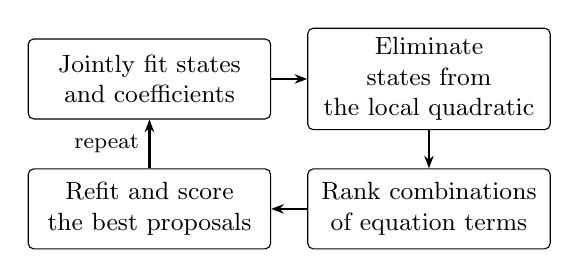
\begin{tikzpicture}[box/.style={draw,rounded corners=2pt,align=center,text width=1.12in,minimum height=0.40in,font=\small},arr/.style={-{Stealth[length=1.6mm]},thick}]
\node[box] (fit) at (0,0) {Jointly fit states\\and coefficients};
\node[box] (profile) at (3.55,0) {Eliminate states from\\the local quadratic};
\node[box] (search) at (3.55,-1.65) {Rank combinations\\of equation terms};
\node[box] (refit) at (0,-1.65) {Refit and score\\the best proposals};
\draw[arr] (fit)--(profile);\draw[arr] (profile)--(search);
\draw[arr] (search)--(refit);\draw[arr] (refit)--node[left,font=\footnotesize]{repeat}(fit);
\end{tikzpicture}
\captionof{figure}{PJSS alternates support proposals and nonlinear joint fits. Enumeration is per equation within a size limit; the nonlinear search is not globally exhaustive.}
\label{fig:method}
\end{center}

\lead{Profile out state adjustments.} At the current fit, form the Gauss--Newton blocks over all coefficients, including inactive terms. Eliminating state increments yields
\begin{equation}
 H=A_{cc}-A_{uc}^{\top}A_{uu}^{-1}A_{uc},\quad
 g=g_c-A_{uc}^{\top}A_{uu}^{-1}g_u.
 \label{eq:profile}
\end{equation}
The quadratic is $q(\delta c)=\delta c^\top H\delta c+2g^\top\delta c$, with small diagonal regularization. Profiling accounts for local trajectory adjustment when coefficients change, without solving the nonlinear state problem for each support.

\lead{Search combinations, then refit.} After projecting out other equations' active columns, we rank subsets of up to five terms per equation: 21,699 nonempty subsets for $M=20$, plus the empty support. The best two per size supply replacements and combinations across equations. The ten best unfitted proposals receive nonlinear fits, for at most two rounds. Larger libraries use beam search.

\lead{Select sparsity from the data.} A BIC-inspired score adds observation and dynamics losses to a complexity penalty. Degree-$d$ terms cost $\log(Dn)\max\{0.1,1+0.2(d-1.5)\}$ with autocorrelation corrections. Every third observation is masked during candidate fitting and included in scoring. Because preprocessing still uses these samples, this is not independent temporal validation.

Joint estimation and state elimination are established ingredients. Profiled smoothing approximations also predate this work~\cite{zhang}. Section~\ref{sec:ablation} isolates the contribution of profiling within PJSS.
\end{minipage}

% PAGE 2: two wide scientific figures and the equations actually fitted.
\clearpage
\section{Actual predictions and recovered equations}
\centering
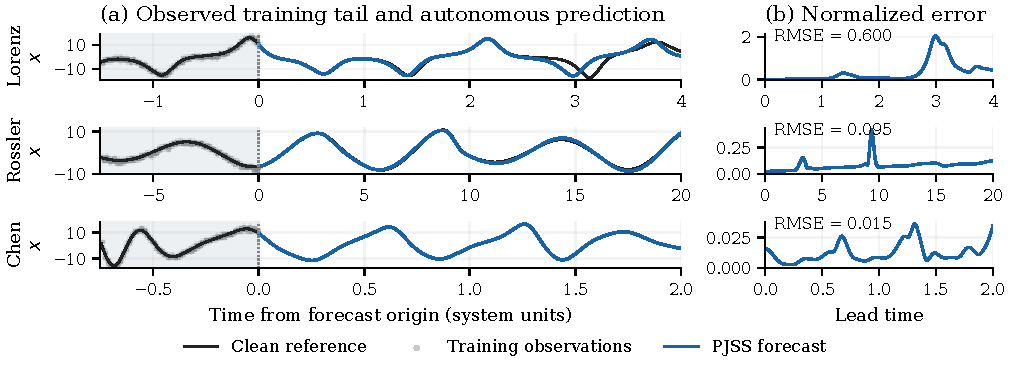
\includegraphics[width=0.98\textwidth]{figures/predictions.pdf}
\captionof{figure}{\textbf{Held-out prediction after fitting noisy observations.} Models fit 2,000 samples with 10\% Gaussian noise; the next 400 targets are withheld. Gray dots show training observations. Forecasts use learned coefficients and a state estimated from the final 40 training observations, with no clean initialization. Left: $x$; right: instantaneous error over all coordinates, normalized by clean training standard deviations. Annotations report full-horizon RMSE.}
\label{fig:predictions}
\vspace{6pt}
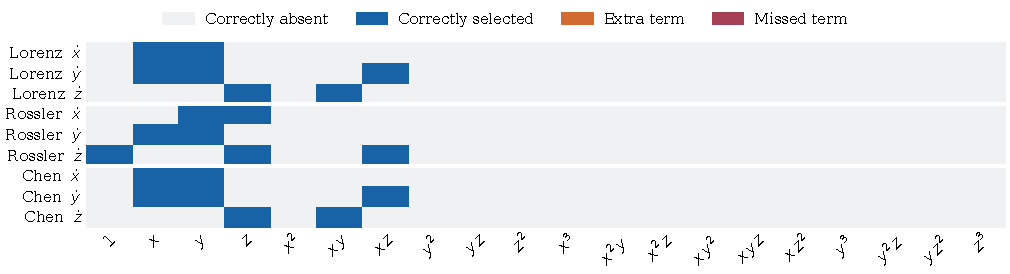
\includegraphics[width=0.90\textwidth]{figures/support.pdf}
\captionof{figure}{\textbf{Sparse discovery in the same models.} Rows: 20 candidate monomials; columns: equations. Blue: correctly selected; gray: correctly absent. All cases recover seven of seven terms with no extras. Coefficient error is $\|\hat C-C\|_F/\|C\|_F$. These fixed illustrations do not estimate benchmark accuracy.}
\label{fig:support}
\par\vspace{7pt}
\noindent\begin{minipage}[t]{0.478\textwidth}\vspace{0pt}

\lead{A fitted equation, not just a support score.} The Lorenz run in Figures~\ref{fig:predictions}--\ref{fig:support} returns
\begin{equation}
\begin{aligned}
 \dot x&=\LorenzEqX,\\
 \dot y&=\LorenzEqY,\\
 \dot z&=\LorenzEqZ.
\end{aligned}
\label{eq:lorenz}
\end{equation}
Reference coefficients are $(-10,10)$, $(28,-1,-1)$ and $(-8/3,1)$. Display rounding is not used in integration.

\lead{Fixed cases.} Default PJSS v1.2 fits one run per system, using seed 20261105 and a 1,000-sample burn. Cases were specified before fitting; no outcome-based replacement was made. They are separate from historical benchmarks.

\end{minipage}\hfill
\begin{minipage}[t]{0.478\textwidth}\vspace{0pt}
\noindent\textbf{Prediction error across coordinates.}
\begin{center}\small
\begin{tabular}{@{}lrrr@{}}\toprule
System & $\Delta t$ & First 100 & All 400\\\midrule
Lorenz & 0.010 & \LorenzShort & \LorenzLong\\
R\"ossler & 0.050 & \RosslerShort & \RosslerLong\\
Chen & 0.005 & \ChenShort & \ChenLong\\\bottomrule
\end{tabular}
\end{center}
\noindent RMSE normalizes each coordinate by its clean training standard deviation. Horizons differ in physical time across systems. Truth generates and scores data but does not select supports or initialize forecasts.

Lorenz's error grows despite correct terms and a coefficient error of \LorenzCoef\%. Figure~\ref{fig:attractors} examines geometry separately: a similar attractor does not establish equality of invariant distributions.
\end{minipage}

% PAGE 3: attractors across the full width, aggregate recovery below.
\clearpage
\centering
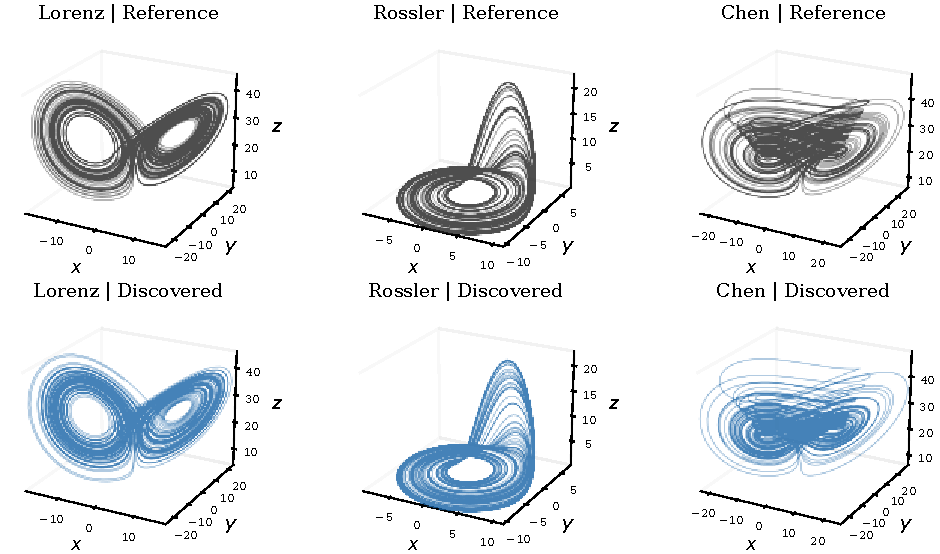
\includegraphics[width=0.91\textwidth]{figures/attractors.pdf}
\captionof{figure}{\textbf{Attractors generated by the discovered equations.} Top: reference; bottom: learned models from Figures~\ref{fig:predictions}--\ref{fig:support}. Each is an autonomous 8,000-sample integration after a 1,000-sample burn, starting from the estimated training endpoint. Axis limits match within systems; sample intervals match the prediction table. No observations are assimilated. Geometry is a qualitative check, not a test of invariant statistics or long-horizon forecast accuracy.}
\label{fig:attractors}
\par\vspace{8pt}
\noindent\begin{minipage}[t]{0.478\textwidth}\vspace{0pt}

\section{Recovery across systems}
\lead{External benchmark.} \texttt{dysts}~\cite{dysts} supplies 77 in-library systems: 61 three-dimensional (degree $\le3$) and 16 of dimension 4--6 (degree $\le2$). Its 6,160 runs cross $N\in\{500,2000\}$, four noise levels (1--20\%) and ten replicates. Forty-nine systems are outside development benchmarks; others overlap or share a support.

Exact recovery is 89.0\% overall and 85.3\% on new systems; system-resampled 95\% intervals are 84.1--93.1\% and 78.3--91.4\%. All equations must have the correct terms. Fifty-six systems reach 90\% recovery; five fall below 50\%. Small terms and fast dynamics remain difficult.

\begin{center}
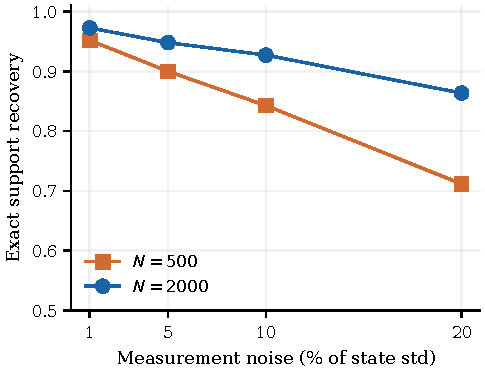
\includegraphics[width=\linewidth]{figures/recovery_noise.pdf}
\captionof{figure}{\textbf{Recovery under increasing measurement noise.} PJSS on all 77 \texttt{dysts} systems; each point averages 770 trajectories. These are historical frozen-model results, separate from the three new illustrations.}
\label{fig:noise}
\end{center}

\end{minipage}\hfill
\begin{minipage}[t]{0.478\textwidth}\vspace{0pt}
\lead{Comparison with DEDi.} We use the authors' code and the full 35-setting grid. A first paired study contains 80 runs across five conditions on core system families: white, coloured and heavy-tailed noise, short records, and a high-noise stress condition. A second contains 64 runs from 35 new three-dimensional systems. Protocols were recorded in the repository before these comparisons.

\begin{center}\small
\begin{tabular}{@{}lrr@{}}\toprule
Method / selection & Core & New\\
 & $n=80$ & $n=64$\\\midrule
\textbf{PJSS} & \textbf{66} & \textbf{53}\\
DEDi / validation & 55 & 36\\
DEDi / BIC & 61 & 41\\\bottomrule
\end{tabular}
\captionof{table}{Exact recoveries under full-grid comparison. The studies use different system sets; counts are not pooled.}
\label{tab:dedi}
\end{center}

On core systems, 66 versus 61 does not establish superiority over DEDi-BIC. Excluding coloured noise, both recover 56/64. On new systems, PJSS has 15 paired wins and three losses against DEDi-BIC. A post-hoc system bootstrap gives a 95\% interval of 4.4--34.4 percentage points for the PJSS advantage. The difference is concentrated at 1--5\% noise (29/32 versus 19/32); at 10--20\% the counts are 24/32 versus 22/32.
\end{minipage}

% PAGE 4: interpretation, reproducibility and references.
\clearpage
\noindent\begin{minipage}[t]{0.478\textwidth}\vspace{0pt}
\section{Which components matter?}
\label{sec:ablation}
Ablations use 576 paired runs: white noise (160), coloured noise (89), a high-noise stress set (40), and three-dimensional \texttt{dysts} (287).

\begin{center}
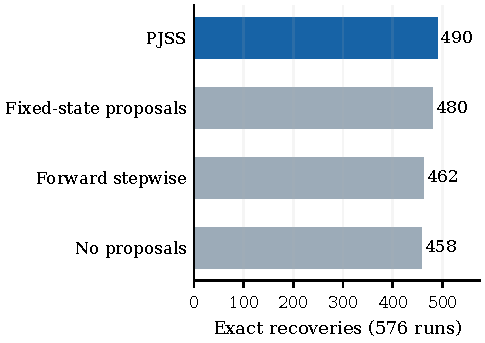
\includegraphics[width=\linewidth]{figures/ablation.pdf}
\captionof{figure}{\textbf{Separating search from profiling.} Removing proposals or replacing subset enumeration with forward stepwise search loses more recoveries than keeping enumeration but holding states fixed during the proposal step. All variants retain joint nonlinear refits.}
\label{fig:ablation}
\end{center}

Removing proposals loses 32 recoveries and gains none; replacing enumeration with forward stepwise selection loses 28 and gains none. On the hard 40, refitting all starts without proposals recovers 19, against 28 for the full search. Support changes are central to the gain.

Fixed-state proposals retain exhaustive subsets and nonlinear refits. PJSS recovers 490/576 against 480/576, with 15 paired wins and five losses. The fixed-state variant wins one more coloured-noise case. Profiling adds a smaller, setting-dependent gain.

\lead{Noise calibration.} Correlated errors can be overfit as dynamics. Changing the AR(1) residual loss to Gaussian raises recovery from 75.4\% to 80.5\% on a fresh 800-run coloured archive (43 paired wins, two losses), leaving white and heavy-tailed paths unchanged.

\lead{Cost.} In three separately timed cases, PJSS takes about five seconds per run; full-grid DEDi takes 501--4,462 seconds with one GPU process. Two cases are Sprott A and one Rabinovich--Fabrikant. Different execution setups and this small sample preclude a universal speedup claim. Subset enumeration still grows combinatorially with library size.

\lead{Versions.} New illustrations and DEDi comparisons use v1.2. Aggregate \texttt{dysts} results retain the earlier frozen model; refinements change its rate by about 0.1 percentage point. Some test findings informed subsequent development, followed by fresh confirmations. The project is not one untouched test pass.

\end{minipage}\hfill
\begin{minipage}[t]{0.478\textwidth}\vspace{0pt}
\section{Limitations and conclusions}
\lead{Scope.} Positive results assume uniform sampling, full observation and an in-library generating model. Process noise, irregular sampling and unknown forcing remain unvalidated. The prior favors low-degree equations. Runs nest within systems, limiting inference from run-level comparisons.

\lead{Local search.} Proposals use a local quadratic, at most five terms per equation and two rounds. Larger libraries use beam search. The ambiguity flag does not certify correctness. AR(1) handling is restricted to three dimensions; higher-dimensional tests use degree-two libraries.

\lead{Measured-data failures.} A single pendulum fails the prescribed support criterion, although dependent embedding terms complicate that metric. A double pendulum has out-of-library rational dynamics: forecasts are worse than SINDy baselines and the ambiguity flag remains silent. Figure~\ref{fig:attractors} also does not test invariant measures, spectra or Lyapunov exponents.

\lead{Reproducibility.} Affected historical weak-baseline comparisons are omitted because of a seeding issue. Main archives are available locally; four secondary-study originals are missing. Public artifact release and the original benchmark environment remain tasks. The new figures preserve inputs, coefficients, initialization and integration settings.

PJSS connects support search to joint state estimation. Synthetic tests and the new predictions support in-library recovery; measured and misspecified systems remain open challenges.

\begin{thebibliography}{6}
\small
\bibitem{sindy} S.~L. Brunton, J.~L. Proctor, and J.~N. Kutz. Discovering governing equations from data by sparse identification of nonlinear dynamical systems. \emph{PNAS}, 113:3932--3937, 2016.
\bibitem{weak} D.~A. Messenger and D.~M. Bortz. Weak SINDy: Galerkin-based data-driven model selection. \emph{Multiscale Modeling \& Simulation}, 19:1474--1497, 2021.
\bibitem{sidds} J.~M. Hokanson, G.~Iaccarino, and A.~Doostan. Simultaneous identification and denoising of dynamical systems. \emph{SIAM J. Scientific Computing}, 45:A1413--A1437, 2023.
\bibitem{dedi} T.~Meissner and K.~Glasner. Simultaneous model discovery and state estimation under high data corruption. \emph{SIAM J. Applied Dynamical Systems}, 25:1439--1467, 2026.
\bibitem{zhang} X.~Zhang, J.~Cao, and R.~J. Carroll. On the selection of ordinary differential equation models with application to predator-prey dynamical models. \emph{Biometrics}, 71:131--138, 2015.
\bibitem{dysts} W.~Gilpin. Chaos as an interpretable benchmark for forecasting and data-driven modelling. \emph{NeurIPS Datasets and Benchmarks}, 2021.
\end{thebibliography}
\end{minipage}
\end{document}
